\documentclass{beamer}

\usepackage{beamerthemesplit}
\usetheme{Singapore} %Copenhagen}

\input{../../include/preamble.inc} 
\input{../../include/definitions.inc} 
\input{../../include/author.inc} 

\title[]{Течения вязкой жидкости}

\begin{document}
	
\frame[plain]{\titlepage}


\frame[plain]{
	\frametitle{Аннотация}
	\parbox{\textwidth}{
	Понятие вязкой жидкости. Тензор напряжений для вязкой несжимаемой жидкости. Система уравнений Навье -- Стокса. Постановка граничных условий. Подобие течений вязкой несжимаемой жидкости. $\Pi$-теорема. Течение Пуазейля.
	}
}

\frame{
	\frametitle{Понятие вязкой жидкости}
	
	\begin{columns}
		\begin{column}{0.4\textwidth}
			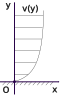
\includegraphics[width=\linewidth]{../img/visc_def.pdf}
		\end{column}
		\begin{column}{0.6\textwidth}
			\begin{exampleblock}{Касательная сила, действующая на стенку}
				\parbox{\textwidth}{
					\[
					\tau= \mu \od{v}{y} = \rho\nu \od{v}{y},
					\]
					где $\mu=\rho\nu$ -- коэффициент динамической вязкости;
					$\nu$ --  коэффициент кинематической вязкости; $\rho$ -- плотность.
					

				}
			\end{exampleblock}\pause
		
			\begin{exampleblock}{Размерность коэффициентов вязкости}
				\parbox{\textwidth}{
				\[
					[\mu] = \frac{\text{кг}}{\text{м} \cdot \text{с}},\quad
					[\nu] = \frac{\text{м}^2}{\text{с}}.
				\]
					
				}
			\end{exampleblock}
		
			
		\end{column}
	\end{columns}
}


\frame{
	\frametitle{ Тензор напряжений вязкой несжимаемой жидкости }
	
	\begin{columns}
		\begin{column}{0.3\textwidth}
			\centering\scriptsize
			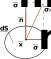
\includegraphics[width=\linewidth]{../img/sigma_decomposition}\\
			
			\medskip
			Разложение напряжения, возникающего в сплошной среде, на тангенциальную и нормальную составляющие
		\end{column}
		\begin{column}{0.7\textwidth}
				\begin{exampleblock}{Связь тензора напряжений и тензора скоростей деформаций}
				\parbox{\textwidth}{
					\[
					\sigma = -pI + 2\mu e,
					\]
					где $p$ -- давление; $I$ -- единичный тензор; $e$ -- тензор скоростей деформаций, задаваемый соотношением
					\[
					e_{ij} = \frac{1}{2}\left( \pd{v_i}{x_j}+\pd{v_j}{x_i} \right),
					\]
					где $v_i$  -- компоненты вектора скорости ($i=1,2,3$).
				}
			\end{exampleblock}
		\end{column}
	\end{columns}
	

	
}

\frame{
	\frametitle{ Уравнения движения вязкой несжимаемой жидкости }
	
	\begin{exampleblock}{Уравнения Навье -- Стокса}
		\parbox{\textwidth}{
			\[
				\divo \vec{v} = 0,
			\]
			\[
				\pd{\vec{v}}{t} + (\vec{v}\cdot\nabla)\vec{v} = -\frac{1}{\rho}\nabla p + \nu \Delta \vec{v} + \vec{f},
			\]
			\[
			c_V\left(\pd{T}{t} + (\vec{v}\cdot\nabla)T \right) = \frac{\kappa}{\rho} \Delta T + \frac{2\mu}{\rho} e_{ij}e_{ij}.
			\]
			
			\medskip
			\alert{Неизвестные функции}, определенные и дифференцируемые в некоторой области пространства:  $\vec{v}\argtxv$ -- вектор скорости; $p\argtxv$ -- давление; $T\argtxv$ -- температура. 

			\medskip			
			\alert{Константы}: $\rho$ -- плотность; $\nu$ -- коэффициент кинематической вязкости; $\kappa$ -- коэффициент температуропроводности.
			
			\medskip
			\alert{Обозначения}: $e_{ij}$ -- компоненты тензора скоростей деформаций; $\vec{f}$ -- вектор внешних сил.
			
		}
	\end{exampleblock}
}

\frame{
	\frametitle{Уравнения движения вязкой несжимаемой жидкости}
	
	\parbox{\textwidth}{
	Система уравнений разбивается на две подсистемы:	
	}
	
	
	\begin{exampleblock}{Уравнения Навье -- Стокса}
		\parbox{\textwidth}{
		\[
		\divo \vec{v} = 0,
		\]
		\[
		\pd{\vec{v}}{t} + (\vec{v}\cdot\nabla)\vec{v} = -\frac{1}{\rho}\nabla p + \nu \Delta \vec{v} + \vec{f}.
		\]	
		}
	\end{exampleblock}

	\begin{exampleblock}{Закон динамики температуры}
		\parbox{\textwidth}{
		\[
		c_V\left(\pd{T}{t} + (\vec{v}\cdot\nabla)T \right) = \frac{\kappa}{\rho} \Delta T + \frac{2\mu}{\rho} e_{ij}e_{ij}
		\]	
		}
	\end{exampleblock}	
	
	\parbox{\textwidth}{
		Решив уравнения Навье -- Стокса, мы найдем распределение ско\-рос\-ти и давления. Зная распределение скорости, из второй части находим распределение температуры. Дальше будут рассматриваться решения только первой части, т.е. уравнений Навье -- Стокса.
	}
	
	
}

\frame{
	\frametitle{Граничные условия для уравнения Навье -- Стокса}
	
	\begin{columns}
		\begin{column}{0.5\textwidth}
			\begin{exampleblock}{Условия на неподвижной границе}
			\parbox{\textwidth}{
			\centering
			\medskip
			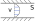
\includegraphics[width=0.7\linewidth]{../img/motionless_bound}

			\bigskip
			Кинематическое условие:
			\[
			\vec{v}|_S = 0.
			\]

			}
			\end{exampleblock}
			\smallskip
		\end{column}\pause
	
		\begin{column}{0.5\textwidth}
			\begin{exampleblock}{Условие на подвижной границе}
				\parbox{\textwidth}{
					
					\centering
					\medskip
					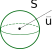
\includegraphics[width=0.5\linewidth]{../img/moving_rigid_bound}
					
					\bigskip
					Кинематическое условие:
					\[
					\vec{v}|_S = \vec{u}.
					\]
					
				}
			\end{exampleblock}
			
		\end{column}
	\end{columns}\pause
	
	\parbox{\textwidth}{
	\centering
	Такого вида граничные условия называются условиями \alert{<<прилипания>>}.
	}
	
	
}

\frame{
	\frametitle{Граничные условия для уравнения Навье -- Стокса}
	
	\begin{exampleblock}{Условия на свободной границе}
		\parbox{\textwidth}{
		\begin{columns}
			\begin{column}{0.5\textwidth}
				\scriptsize
				\centering
				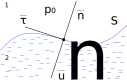
\includegraphics[width=0.7\linewidth]{../img/free_bound}
				
				\medskip
				1 -- газ; 2 -- вязкая жидкость
			\end{column}
			\begin{column}{0.5\textwidth}
			Кинематическое условие:
			\[
			v_n|_S = u_n.
			\]
			
			\medskip
			Динамические условия:
			\[
			(\vec{n}\cdot\sigma)\cdot\vec{n}|_S= p|_S = p_0,
			\]
			\[
			(\vec{n}\cdot\sigma)\cdot\vec{\tau}|_S = 0.
			\]

				
			\end{column}
		\end{columns}	
		}
	\end{exampleblock}
	
}




\frame{
	\frametitle{Подобие при течениях вязкой несжимаемой жидкости}
	
	\begin{exampleblock}{Определение}
		\parbox{\textwidth}{
			Два физических явления называются \alert{подобными}, если величины, характеризующие одно явление, могут быть получены из соответствующих величин другого, взятых в сходственных пространственно-временных точках, простым умножением на \textit{одинаковые во всех точках множители}, называемые \textit{коэффициентами подобия}.
		}
	\end{exampleblock}
}


\frame{
	\frametitle{Подобие при течениях вязкой несжимаемой жидкости}
		\begin{exampleblock}{Уравнения Навье -- Стокса в декартовой системе координат}
		\parbox{\textwidth}{
					
	\[
	\pd{v_x}{x}+\pd{v_y}{y}+\pd{v_z}{z} = 0,
	\]
	\[
	\pd{v_x}{t} + 
	v_x \pd{v_x}{x} + v_y \pd{v_x}{y} + v_z \pd{v_x}{z} = 
	X -\frac{1}{\rho}\pd{p}{x} + 
	\nu \left(\pdk{v_x}{x} + \pdk{v_x}{y}+ \pdk{v_x}{z} \right),
	\]
	\[
	\pd{v_y}{t} + 
	v_x \pd{v_y}{x} + v_y \pd{v_y}{y} + v_z \pd{v_y}{z} = 
	Y -\frac{1}{\rho}\pd{p}{y} + 
	\nu \left(\pdk{v_y}{x} + \pdk{v_y}{y}+ \pdk{v_y}{z} \right),
	\]
	\[
	\pd{v_z}{t} + 
	v_x \pd{v_z}{x} + v_y \pd{v_z}{y} + v_z \pd{v_z}{z} = 
	Z -\frac{1}{\rho}\pd{p}{z} + 
	\nu \left(\pdk{v_z}{x} + \pdk{v_z}{y}+ \pdk{v_z}{z} \right).
	\]
	
		}
	
		\end{exampleblock}
}

\frame{
	\frametitle{Подобие при течениях вязкой несжимаемой жидкости }
	
	\begin{exampleblock}{Замена переменных}
		\parbox{\textwidth}{
			\[
			t = T t',\quad
			x = L x',\quad 
			y = L y',\quad
			z = L z',			
			\]
			\[
			v_x = V v_x',\quad
			v_y = V v_y',\quad
			v_z = V v_z',\quad
			p = P p',
			\]
			\[
			X = F X',\quad
			Y = F Y',\quad
			Z = F Z',
			\]
			где $T$, $L$, $V$, $P$, $F$ -- характерные значения времени, размера течения, скорости, давления, силы сплошной среды. 
			
			Штрихами обозначены новые безразмерные переменные. 
			
			
		}
	\end{exampleblock}
	
}



\frame{
	\frametitle{Подобие при течениях вязкой несжимаемой жидкости}
	
	\begin{exampleblock}{Уравнения Навье -- Стокса, записанные с использованием безразмерных комплексов}
	\parbox{\textwidth}{
	\small

	\[
		Sh\pd{v'_x}{t'} + 
		v_x' \pd{v_x'}{x'} + v_y' \pd{v_x'}{y'} + v_z' \pd{v_x'}{z'} = 
		\frac{1}{Fr} X' - Eu \pd{p'}{x'} + 
		\frac{1}{Re} \left(\pdk{v_x'}{x'} + \pdk{v_x'}{y'}+ \pdk{v_x'}{z'} \right),
	\]
	\[
		Sh\pd{v_y'}{t'} + 
		v_x' \pd{v_y'}{x'} + v_y' \pd{v_y'}{y'} + v_z' \pd{v_y'}{z'} = 
		\frac{1}{Fr} Y' - Eu \pd{p'}{y'} + 
		\frac{1}{Re} \left(\pdk{v_y'}{x'} + \pdk{v_y'}{y'}+ \pdk{v_y'}{z'} \right),
	\]
	\[
		Sh\pd{v_z'}{t'} + 
		v_x \pd{v_z'}{x'} + v_y' \pd{v_z'}{y'} + v_z' \pd{v_z'}{z'} = 
		\frac{1}{Fr} Z' - Eu \pd{p'}{z'} + 
		\frac{1}{Re} \left(\pdk{v_z'}{x'} + \pdk{v_z'}{y'}+ \pdk{v_z'}{z'} \right).
	\]
			
	}
	\end{exampleblock}

	\begin{exampleblock}{Безразмерные комплексы -- критерии подобия }
		\centering	\small
		\parbox{0.8\textwidth}{
			
			\begin{tabular}{ll}
			$\displaystyle\frac{L}{VT} = \Sh$ -- число Струхаля, & $\displaystyle\frac{P}{\rho V^2}=\Eu$ -- число Эйлера, \\
			$\displaystyle\frac{VL}{\nu} = \Re$ -- число Рейнольдса, & $\displaystyle\frac{V^2}{F L}=\Fr$ -- число Фруда.
			\end{tabular}
			
			
		}
	\end{exampleblock}
	
}

\frame{
	\frametitle{Колебание струн в однородном потоке воздуха }
	

	\centering
	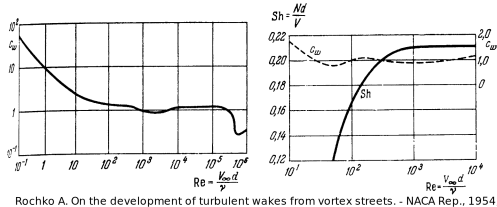
\includegraphics[width=0.85\textwidth]{../img/Sh_tube_tr.png}	
	
	
	\begin{exampleblock}{Критерии подобия}
		\parbox{\textwidth}{
			\[
			\Sh = \Sh(\Re) = \frac{N d}{V_\infty},\quad
			c_w = \Eu(\Re) = \frac{P}{\rho V_\infty^2},\quad
			\Re = \frac{V_\infty d}{\nu}.
			\]
			\textit{Заданные величины}: $d$ -- диаметр струны; $V_\infty$ -- скорость набегающего потока; $\nu$ -- вязкость; $\rho$ -- плотность.\\ \textit{Неизвестные}: $N$ -- частота колебаний; $P$ -- давление.
		}
	\end{exampleblock}
}

\frame{
	\frametitle{Основы теории размерности}

	\begin{exampleblock}{Определение}
	\parbox{\textwidth}{
		Функция $f(x_1, x_2, \ldots, x_n)$ называется \alert{размернооднородной}, если существует такая совокупность чисел $b_k$ ($k=\overline{1,m}$), что имеет место равенство
		\[
		f(\alpha_1^{a_{11}}\ldots \alpha_m^{a_{1m}}x_1,\ldots,
		\alpha_1^{a_{n1}}\ldots \alpha_m^{a_{nm}}x_n) = 
		\alpha_1^{b_1}\alpha_2^{b_2}\ldots \alpha_m^{b_m} f(x_1, x_2, \ldots, x_n)
		\]	
		для всех $\alpha_k$ ($k=\overline{1,m}$) и $x_i$ ($i=\overline{1,n}$) в области определения.
	}
	\end{exampleblock}	
}


\frame{
	\frametitle{Основы теории размерности}
	
	
	\begin{exampleblock}{$\Pi$-теорема (Бекингем, Федерман)}
		\parbox{\textwidth}{
			Если $x_1$, $x_2$, \ldots, $x_n$ -- численные значения $n$ физических величин, $A=(a_{ij})$ ($i=\overline{1,n}$, $j=\overline{1,m}$) -- матрица их размерностей по отношению к единицам измерения $M_1$, $M_2$,\ldots, $M_m$, $f$ -- произвольная размернооднородная функция переменных  $x_1$, $x_2$, \ldots, $x_n$, а $\Pi_1$, $\Pi_2$, \ldots, $\Pi_p$ ($p=n-r$, $r$ -- ранг матрицы $A$) -- фундаментальная система степенных одночленов переменных $x_1$, $x_2$, \ldots, $x_n$, то при произвольных действительных числах $k_1$, $k_2$, \ldots, $k_n$ имеет место равенство
			\[
			f(x_1, x_2, \ldots, x_n) = x_1^{k_1} x_2^{k_2} \ldots x_n^{k_n}
			G(\Pi_1, \Pi_2, \ldots, \Pi_p).
			\]
		}
	\end{exampleblock}


}

\frame{
	\frametitle{ Основы теории размерности }
	
	\begin{columns}
		\begin{column}{0.5\textwidth}
		\begin{exampleblock}{Размерности параметров в уравнениях Навье -- Стокса}
			\parbox{\textwidth}{
			\[
			\begin{array}{c||rrr||}
			& \text{кг} & \text{м} & \text{с}\\
			\hline
			x,y,z & 0 & 1 & 0\\
			t     & 0 & 0 & 1\\
			u,v,w & 0 & 1 & -1\\
			p     & 1 & -1 & -2\\
			g     & 0 & 1 & -2\\
			\rho  & 1 & -3 & 0\\
			\mu   & 1 & -1 & -1
			\end{array}
			\]	
			}
		\end{exampleblock}
		\end{column}
		\begin{column}{0.5\textwidth}
		\parbox{\textwidth}{
			Ранг матрицы $r=3$. Число размерных величин, определяющих движение, равно 7. Фундаментальная система параметров $\Pi$ содержит $p=n-r=4$ параметра. Это, например, ранее введенные \alert{числа подобия $\Re$, $\Sh$, $\Eu$, $\Fr$}.
			

		}
	
		\end{column}
	\end{columns}

\begin{exampleblock}{Общее решение уравнений Навье -- Стокса без учета краевых и начальных условий}
	\parbox{\textwidth}{
		\[
		f(x_1, x_2, \ldots, x_n) = x_1^{k_1} x_2^{k_2} \ldots x_n^{k_n}
		G(\Re, \Fr, \Sh, \Eu)
		\]
	}
\end{exampleblock}


}

\frame{
	\frametitle{Течение Пуазейля}
	
	\centering
	\includegraphics[width=0.7\linewidth]{../img/Poiseuille}

	
	\begin{exampleblock}{Постановка задачи}
		\parbox{\textwidth}{
			В трубе постоянного сечения под действием перепада давления $\Delta p = p_2-p_1$ течет жидкость плотности $\rho$ и вязкостью $\nu$. Требуется найти кинематические и динамические характеристики потока.
		}
	\end{exampleblock}
}


\frame{
	\frametitle{Постановка математической задачи}
	\parbox{\textwidth}{
	Ищем решение стационарных уравнений Навье -- Стокса в виде:
	\[
		p=p(x,y,z), \quad \vec{v} = v(x,y,z)\vec{e}_z.
	\]	
	
	Система уравнений, спроектированная на оси координат:
	\[
	\pd{v}{z} = 0,\quad
	0 = -\frac{1}{\rho}\pd{p}{x},\quad
	0 = -\frac{1}{\rho}\pd{p}{y},
	\]
	\[
	v\pd{v}{z} = -\frac{1}{\rho}\pd{p}{z} + 
	\nu \left(\pdk{v}{x}+\pdk{v}{y}+\pdk{v}{z}\right).
	\]
	
	Условия на границах:
	\[
	p|_{z=0} = p_2,\quad p|_{z=L} = p_1,
	\]
	\[
	v|_S = 0,
	\]
	где $S$ -- поверхность трубы. 
	}
	
}

\frame{
	\frametitle{Течение Пуазейля }
	\begin{exampleblock}{Решение}
		\parbox{\textwidth}{
			Так как $\displaystyle\pd{v}{z} = 0$ и $p=p(z)$, то 
			\[
			\pd{p}{z} = \mu \left(\pdk{v}{x}+\pdk{v}{y}\right) = \lambda \quad\Rightarrow\quad
			\lambda  = \frac{p_2-p_1}{L}.
			\]
%			где $\lambda$ -- константа.
			
			Из граничных условий следует решение для давления
			\[
				p(z) = p_2 + \frac{p_1-p_2}{L} z
			\]
			и задача Дирихле для определения профиля скорости
			\[
			\pdk{v}{x}+\pdk{v}{y} = \frac{\Delta p}{\mu L},\quad
			v|_\gamma = 0,
			\]
			где $\gamma$ -- кривая на пересечении поверхности $S$ и плоскости $Oxy$.
		}
	\end{exampleblock}
}

\frame{
	\frametitle{Течение Пуазейля: плоский канал }
	\begin{columns}
		\begin{column}{0.6\textwidth}
			\begin{exampleblock}{Скорость течения}
				\parbox{\textwidth}{
					\[
					v(y) = \frac{\Delta p \cdot h^2}{2\mu L}
					\left[
					1 - \left(\frac{y}{h}\right)^2
					\right],
					\]
					\[
					v_{max} = \frac{1}{2}\frac{\Delta p\cdot  h^2}{\mu L}.
					\]		
				}
			\end{exampleblock}
			
			\begin{exampleblock}{Расход по сечению}
				\parbox{\textwidth}{
					\[
					Q = \int\limits_{-h}^h v(y) dy = \frac{2}{3} \frac{\Delta p\cdot h^3}{\mu L}
					\]
				}
			\end{exampleblock}
			
			\begin{exampleblock}{Средняя скорость по течению}
				\parbox{\textwidth}{
					\[
					v_{avg} = \frac{Q}{2h} = \frac{1}{3} \frac{\Delta p \cdot h^2}{\mu L} =
					\frac{2}{3} v_{max}
					\]
					
				}
			\end{exampleblock}
		\end{column}
		\begin{column}{0.4\textwidth}
			\centering\scriptsize
			\includegraphics[width=0.9\linewidth]{../img/Poiseuille_flat.pdf}\\
			
			\medskip
			Профиль скорости при 
			$\Delta p = 5 \cdot 10^4$~ Па, $h=5$~мм, $L=10$~м, $\mu=1004 \cdot 10^{-6}$~Па$\cdot$с
			
			
		\end{column}
	\end{columns}
	
	
	
}

\frame{
	\frametitle{Течение Пуазейля: плоский канал }
	
	\begin{exampleblock}{Закон сопротивления плоского канала}
		\parbox{\textwidth}{
			Вводя коэффициент сопротивления $\lambda$ для плоского канала
			\[
			\Delta p = \lambda \frac{L}{2h} \frac{\rho v_{avg}^2}{2},
			\]
			получим выражение для коэффициента сопротивления через число Рейнольдса:
			\[
			\lambda = \frac{24}{\Re},
			\]
			где 
			$\Re = \displaystyle\frac{v_{avg} 2h}{\nu}$.
		}
	\end{exampleblock}
	
}

\frame{
	\frametitle{ Течение Пуазейля: эллиптический канал }
	
	%	\begin{columns}
	%		\begin{column}{0.65\textwidth}
	\begin{exampleblock}{Скорость течения}
		\parbox{\textwidth}{
			\[
			v(x,y) = \frac{\Delta p }{2\mu L}
			\frac{a^2b^2}{a^2+b^2}
			\left(
			1 - \frac{x^2}{a^2} - \frac{y^2}{b^2}
			\right),
			\]
			\[
			v_{max} = \frac{\Delta p}{2 \mu L} \frac{a^2b^2}{a^2+b^2}.
			\]		
		}
	\end{exampleblock}
	
	\begin{exampleblock}{Расход по сечению}
		\parbox{\textwidth}{
			\[
			Q = \int\limits_{S} v(x,y) dx dy = \frac{1}{2} \pi a b v_{max}
			\]
		}
	\end{exampleblock}
	
	\begin{exampleblock}{Средняя скорость по течению}
		\parbox{\textwidth}{
			\[
			v_{avg} = \frac{Q}{\pi a b} = \frac{1}{2} v_{max}
			\]
			
		}
	\end{exampleblock}
}

\frame{
	\frametitle{ Течение Пуазейля: круглый канал }
	
		\begin{columns}
		\begin{column}{0.65\textwidth}
			\begin{exampleblock}{Скорость течения}
				\parbox{\textwidth}{
					\[
					v(x,y) = \frac{\Delta p }{2\mu L}
					\frac{r^2}{2}
					\left(
					1 - \frac{x^2+y^2}{r^2} 
					\right),
					\]
					\[
					v_{max} = \frac{\Delta p}{2 \mu L} \frac{r^2}{2}.
					\]		
				}
			\end{exampleblock}
			
			\begin{exampleblock}{Расход по сечению}
				\parbox{\textwidth}{
					\[
					Q = \int\limits_{S} v(x,y) dx dy = \frac{1}{2} \pi r^2 v_{max}
					\]
				}
			\end{exampleblock}
			
			\begin{exampleblock}{Средняя скорость по течению}
				\parbox{\textwidth}{
					\[
					v_{avg} = \frac{Q}{\pi r^2} = \frac{1}{2} v_{max}
					\]
					
				}
			\end{exampleblock}
		\end{column}
		\begin{column}{0.45\textwidth}
			\centering\scriptsize
			\includegraphics[width=\linewidth]{../img/Poiseuille_circle.pdf}\\
			
			\medskip
			Профиль скорости при 
			$\Delta p = 5 \cdot 10^4$~ Па, $r=5$~мм, $L=10$~м, $\mu=1004 \cdot 10^{-6}$~Па$\cdot$с
			
			
		\end{column}
	\end{columns}
	
}




\frame{
	\frametitle{Течение Пуазейля: круглый канал }
	
	\begin{exampleblock}{Закон сопротивления круглого канала}
		\parbox{\textwidth}{
			Вводя коэффициент сопротивления $\lambda$ для круглого канала диаметра $d$
			\[
			\Delta p = \lambda \frac{L}{d} \frac{\rho v_{avg}^2}{2},
			\]
			получим выражение для коэффициента сопротивления через число Рейнольдса:
			\[
			\lambda = \frac{64}{\Re}, \,\, \text{где}\,\,
			\Re = \frac{v_{avg} d}{\nu}.
			\]
		}
	\end{exampleblock}
	
}


\frame{
	\frametitle{ Реальное течение в канале }
	
	\centering
	\includegraphics[width=0.7\textwidth]{../img/Reinolds_1.png}

	
}

\frame{
	\frametitle{ Реальное течение в канале }
	
	\centering
	\includegraphics[width=0.7\textwidth]{../img/Reinolds_2.png}
	
	\medskip
	\parbox{\textwidth}{
	\small
	Повторение эксперимента Рейнольдса с краской. Критическое число Рейнольдса $\Re$ в приведенном эксперименте оказалось ниже $13000$ в отличие от оригинального эксперимента Рейнольдса вследствие помех от уличного движения в современном Манчестере.
	
	\medskip
	\scriptsize
	{\em М. Ван-Дайк}. Альбом течений жидкости и газа. М.:Мир, 1986
	}
}

\frame{
	\frametitle{ Литература }
	\begin{literature}[label=]
		\item 
		{\em Лойцянский~Л.~Г.} Механика жидкости газа и плазмы: Учеб. для вузов. --- 7-е изд., испр. -- М.:Дрофа, 2003.
	\end{literature}
}

\end{document}
